\documentclass[11pt,a4paper]{article}
\usepackage[utf8]{inputenc}
\usepackage[ngerman]{babel}
\usepackage{subfigure} 
\usepackage{floatflt}
\usepackage{float}
\usepackage{graphicx}
\usepackage[left=3cm,right=3cm,top=3cm,bottom=3cm]{geometry}
\usepackage{natbib}
\usepackage{wrapfig}
\usepackage{listings}
\usepackage{hyperref}
\usepackage{lineno}
\title{Robotic Games Sommersemester 2019\\ Eine Mauß in 150 Zeilen Code}
\author{Tobias~Bak}

\begin{document}
\maketitle
\section{Problemstellung}
\begin{wrapfigure}{r}{7cm}
\centering
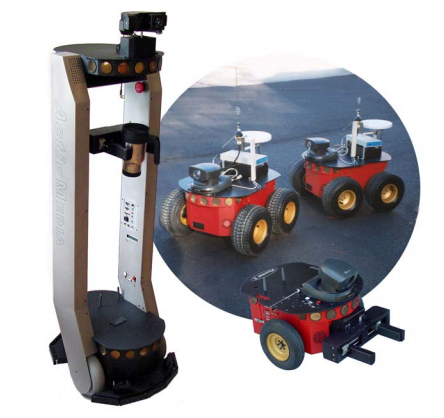
\includegraphics[scale=0.45]{media/titelbild.png}
\caption{Pioneer 3 \cite{pioneer} }
\end{wrapfigure}
Dieses Dokument enthält einen Nachtrag zur Implementierung des Katze und Maus Spiels mit dem Pioneer 3 Roboter.\cite{pioneer}

Als Aufgabe wurde an eine Gruppe von vier Personen die Anforderung den Pioneer Roboter so zu Programmieren dass dieser autonom die Mausrolle eines Katz und Maus spiels zu realisieren. Meine Gruppe hatte die Aufgabe sehr einfach gelöst ohne Verhaltensfusion und ohne reaktiven Verhalten auf die Umgebung. Das Bedeutet der Roboter der unsere Gruppe Programmiert hatte konnte nur hinter einen Vorhang raus und zum Ziel fahren. Die Einfache Implementierung hatte großen Vorteil bei dem Spiel und gewann dieses auch mit Abstand jedoch wurde die Aufgabe nicht in der richtigen Weise gelöst. Aus diesem Grund wurde eine neue Implementierung von Grund auf aufgebaut.
Ziel war es hier auch sich die Randbedingung des Spiels zu nutze zu machen um das Verfahren möglichst elegant und simple zu halten um einerseits Rechenleistung zu sparen und das gesammte System so zu beschleunigen und andererseits eine lange Ausarbeitung zu umgehen, da die hier vorliegende Arbeit nur von mir geschrieben wurde.

Die hier angenommenen Randbedingungen sind dabei die einer bis auf Verstecke konvexer Arena, einer Drehgeschwindigkeit die deutlich größer ist als die Drehgeschwindikgeit sowie bekannter Maße und Farben der Hindernisse, Käsestücke und Katze.

Es war somit möglich das gesammte System in 150 Zeilen zu implementieren aufgeteilt in eine Launch File, ein Skript zur extrahierung optischer Daten, eines zur extrahierung von Sonarbasierten daten sowie der Hauptcode welcher das intelligente Verhalten realisiert.
Es wird hier zunächst mit diesem letzten Teil begonnen, da die Form der in den anderen Programmen generierten Daten auf eben dieses Programm angepasst ist.
\newpage
\section{Fusion Node}
Zunächst soll mit einem Blick auf den Code begonnen werden, welcher hier im folgenden dargstellt ist, der Wichtige Teil ist dabei in Zeilen 7-51 zu sehen.
Im folgenden wird der Code nun durchgegangen und einzelne wichtige Stellen erläutert.

\begin{tiny}
\begin{linenumbers}
\begin{lstlisting}
#!/usr/bin/env python
import sys
import rospy
import numpy as np
from geometry_msgs.msg import Twist
from geometry_msgs.msg import Point
class Fusion:
	def __init__(self):
                # array containes cat,blue,orange,cheese,collision
                self.behaviors = np.zeros((5,2))
                parameters     =  np.array([[-0.5,-1,-1],[0.3,0,1],[0,0,1],[0.8,0,1],[-0.5,-1,-1]])
                for i in range(5):
                    rospy.Subscriber(sys.argv[i+1], Point, self.generate_behavior,
                    (i,parameters[i,0],parameters[i,1],parameters[i,2]))
		self.pub                     = rospy.Publisher('/RosAria/cmd_vel', Twist, queue_size=1)
		while not rospy.is_shutdown():
			self.fusion()
        def generate_behavior(self,msg,args):
                print(args[0])
                if msg.x != 0 and msg.y != 0 :
                    self.behaviors[args[0]] = np.array([1,args[1]*msg.x**args[2]*msg.y**args[3]])
                else:
                    self.behaviors[args[0]] = np.array([1,0])

	def fusion(self):
		#print('collision', self.collision, 'cheese', self.cheese)
		cmd_vel = Twist()
		cmd_vel.linear.x = 1
                cmd_vel.angular.z = prevail_gate(or_gate(
                invoke_gate(self.behaviors[2,1],self.behaviors[0,1]),self.behaviors[3,1]),self.behaviors[4,1])
                #cmd_vel.angular.z = self.behaviors[1,1]
                print(self.behaviors)
		self.pub.publish(cmd_vel)
def and_gate(x, y):
        a = 2.28466
        b = -0.89817
        if x == 0 and y == 0:
            return 0
        else:
            return x*(1-np.exp(-((a*y**2+b*x*y)/(x**2+y**2))))+ y*(np.exp(-((a*x**2+b*x*y)/(x**2+y**2))))
def or_gate(x, y):
        a = 1.02889
        b = 0.3574
        if x == 0 and y == 0:
            return 0
        else:
            return x*(np.exp(-((a*y**2+b*x*y)/(x**2+y**2)))) + y*(np.exp(-((a*x**2+b*x*y)/(x**2+y**2))))
def invoke_gate(x, y):
        return and_gate(or_gate(x, y),x)
def prevail_gate(x, y):
        return or_gate(x, or_gate(x, y))
if __name__ == '__main__':
	try:
		rospy.init_node("fusion")
		fus = Fusion()	
	except rospy.ROSInterruptException:
		rospy.loginfo("---------- FUSION-ERROR! ---------")
\end{lstlisting}
\end{linenumbers}
\end{tiny}
Bei initilalisierung des Programms werden zunächst einzelne Speicher für jedes Verhalten des Roboters zu gewiesen, die hier verwendeten Verhalten sind dabei Verstecken, Fliehen, Käse einsammeln und Kollisionsvermeidung.
Die Einzelnen Verhalten selbst werden dabei im Callback des Subscribers der jeweiligen Messdaten erzeugt.\\
\\
Dabei wird davon Ausgegangen das die eingehenden Daten die Form einer Position relativ zum Roboter haben.
abstrakt kann man nun die Verhalten in 2 Klassen aufteilen: 
Das Regeln dieser Position auf den Sollwert Null und das Regeln auf den Sollwert Unendlich.\\
\\
Aufgrund der langsamen lineargeschwindigkeit des Roboters ist es dabei volkommen ausreichend nur die Drehgeschwindigkeit zu regeln und die lineargeschwindigkeit konstant zu lassen, auch wenn wie im Code zu sehen ist, ein Verhalten immer aus 2 Größen besteht um den Code im Zweifel zu erweitern.
Beide Klassen von Verhalten lassen sich nun mit der \texttt{generate\_behavior} Funktion in Zeilen 18-23 realisieren.
Diese verwendet eine reihe von Inputs welche für jedes Verhalten in Zeile 11 Definiert sind.
Mathematisch implementiert die Funktion die folgende Gleichung für die ausgegebene Geschwindigkeit $v$:
\begin{equation}
	v = p_1*\rho^{p_2}*\phi^{p_3}
\end{equation}
Dabei sind $\rho$ und $\phi$ der Abstand und Winkel zum Roboter und seiner Fahrtrichtung.
für Verhalten welche die Position zu Null regeln wollen führt die Parameter Konfiguration (k,0,1) zu einem Proportionalregler welcher die Orientierung des Roboters so regelt dass er exakt auf das Ziel zu fährt.
Dies ist wie in 11 zu sehen sowohl für die Verstecke als auch den Käse der Fall.
Für das Regeln auf Unendlich wollen wir uns möglichst stark von unserem Ziel wegdrehen, die Drehung sollte dabei stärker sein wenn das Ziel im Zentrum und oder sehr nahe ist, mathematisch erhält man damit die folgende Form:
\begin{equation}
	v= \frac{p_1}{\rho^{p_2}*\phi^{p_3}} ~~~~ p_2,p_3 \textnormal{ungerade}
\end{equation}
Das Regeln zu unendlich kann also mit einer Art proportional Regler mit umgekehrten Vorzeichen in allen Parametern implementiert werden.\\
\\

Wurden die einzelnen Verhalten generiert so werden sie in Zeile 28-36 Fusioniert, diese Fusion folgt \autref{gates} und verwendet die in Zeile 37-54 definierten Analogen Gatter

\begin{figure}[H]
\centering
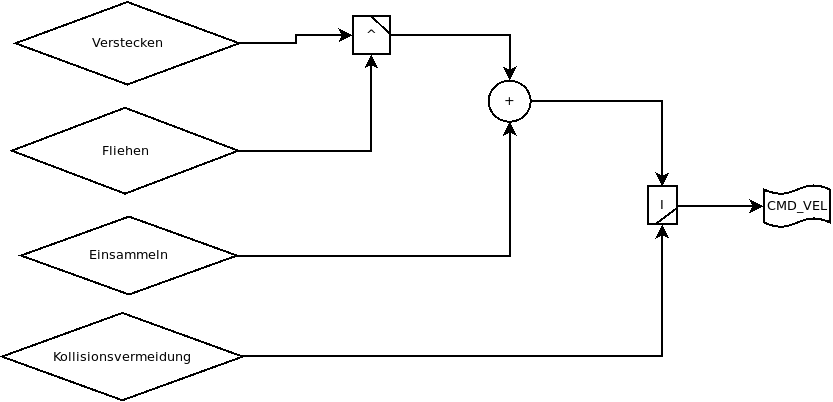
\includegraphics[scale=0.5]{media/gates.png}
\caption{Analogical Gates}\label{gates}
\end{figure}
Anschaulich kann das Verhalten wie folgt verstanden werden:\\
Die Maus versucht zunächst in gleichen Teilen der Katze auszuweichen und den Käse zu erhalten, dies wird über ein analoges OR realisiert was der reinen Winkelgeschwindigkeitsregelung geschuldet ist und dafür sorgt dass sich die Maus nicht immer sofort von der Katze wegdreht, sondern einen großen Bogen um sie fährt.\\
\\
Verstecken wiederum macht nur Sinn wenn man vor der Katze fliehen will und wird entsprechend stärker je stärker der Roboter vor der Katze fliehen will.
Dies wird durch ein INVOKE Gatter realisiert.
Kollisionen sollten selbstverständlich zu jedem Zeitpunkt vermieden werden und so überschreibt die Kollisionsvermeidung jedes andere Verhalten mittels einens PREVAIL Gatters.

Nun da man verstanden hat, wie der Roboter opperiert muss betrachtet werden, wie er die Positionsdaten für die einzelnen Verhalten erhält, hier soll dabei mit den Sonardaten begonnen werden.
\section{Ultraschall}
Das Ultraschallmodul ist zunächst für das Lesen der Ultraschallsensoren zuständig. Aus gelesenen Ultraschalldaten wird eine Position eines zu vermeidendes Objekts für die Verhaltensfusion veröffentlicht. Zusätzlich wird in diesen Modul die Kollisionsvermeidung für das Versteckt ausgeschaltet. Das Modul bindet also nur die Ultraschallsensoren in das Programm ein und berechnet in welchen Winkel sich die kleinste gelesene Distanz befindet und gibt die Entfernung und den Winkel aus. 

Um dies zu ermöglichen benötigt die Node ebenfalls die Entfernungen zu den einzelnen Verstecken.
Die Tatsächliche berechnung passiert im \texttt{sonar\_callback} in Zeilen 80-92.
Zuerst wird $d_o(\alpha)$ berechnet. $d_o(\alpha)$ ist dabei die berechnete Distanz vom Sensor der mit dem Winkel $\alpha$ am Roboter ausgerichtet ist. Die kollisionsvermeidung soll nun unterdrückt werden, wenn sich der Roboter nahe an einem Vorhang befindet, da das Ausweichverhalten mit dem Abstand skaliert, wird dies durch eine modifizierung von $d_o(\alpha)$ zu $d_i(\alpha)$ verwirklicht. Die Idee ist also den Abstand beliebig groß zu stellen, wenn das Versteck beliebig nahe ist, da das entstehende Verhalten so beliebig Schwach wird.
Sei $d_v$ die Vektoren welche die Entfernungen zu beiden Vorhängen beschreibt, dann sind die Ausgabe Distanzen wie folgt definiert (Zeilen 85,86):   
\begin{equation}
d_o(\alpha)=\sqrt{d_i(\alpha)_x^2+d_i(\alpha)_y^2}\cdot 2\cdot(\frac{1}{1+e^{-min(d_v)}}-0,5)
\end{equation}
Anschließend wird der Kleinste Abstand in $d_o$ gesucht und mit dem zugehörigen Winkel zusammen ausgegeben abschließend durch die Verhaltensfusion weiter verarbeitet(Zeilen 87-91). Der Code hierfür sieht wie folgt aus:
  
\begin{scriptsize}
\begin{linenumbers}
\begin{lstlisting} 
#!/usr/bin/env python
import numpy as np
import rospy
from sensor_msgs.msg import PointCloud
from geometry_msgs.msg import Point
max_distance = 1
weight       = np.array([  0.5,   0.7,   1.0,   1.0,  1.0,  1.0,  0.7,  0.5])
sonar_angles = np.array(
[-90.0, -50.0, -30.0, -10.0, 10.0, 30.0, 50.0, 90.0])/ 360.0 * 2 * np.pi
class Sonar:
    def __init__(self):
        self.hideout = np.zeros(2)
        obst_sub  = rospy.Subscriber("/RosAria/sonar",PointCloud,self.sonar_callback)
        blue_sub  = rospy.Subscriber("blue_position",Point,self.hideout_callback,0)
        orang_sub = rospy.Subscriber("orange_position",Point,self.hideout_callback,1)
        while not rospy.is_shutdown():
            print("still working")
    def hideout_callback(self,data,i):
        if data.x != 0:
            self.hideout[i] = data.x
        else:
            self.hideout[i] = 100000
    def sonar_callback(self,data):
        pub       = rospy.Publisher("obstacle_position",Point,queue_size=1)
        sonar_points = data.points
        sonar_ranges = np.zeros(len(sonar_angles))
        for i in range(0, len(sonar_angles)):
            sonar_ranges[i]=np.sqrt(sonar_points[i].x**2+sonar_points[i].y**2)*2*
            (1/(1+np.exp(-1*(min(self.hideout))))-0.5)
        minimum  = np.argmin(sonar_ranges)
        output   = Point()
        if sonar_ranges[minimum] <= max_distance:
            output.x = sonar_ranges[minimum]*weight[minimum]
            output.y = -sonar_angles[minimum]
        pub.publish(output)
if __name__== '__main__':
    rospy.init_node("obstacle_detection")
    try:
        node=Sonar()
    except rospy.ROSInterruptException:
        rospy.loginfo("sonar not working")
\end{lstlisting} 
\end{linenumbers}
\end{scriptsize}
\section{Vision}      
Die Vision ist das Modul um Objekte per Kamera zu erkennen. Es wurde während dieses Projekts nach Farben selektiert, so waren die Katzen Rot, die Vorhänge Gelb und Blau und der Käse Grün. Das Vision Modul sucht abhängig von gewählten Farbe nach Objekten dieser Farbe und Gibt die Entfernung und den Winkel des Objekts aus welchen von der Verhaltensfusion weiter verarbeitet werden.

 Im Ablauf ist das Modul wie folgt aufgebaut. Zunächst wird das Bild in den HSV Farbraum konvertiert (Zeile 117) anschließend werden über das Bild zwei Masken gelegt. Eine Maske schneidet den obere Bildhälfte ab (Zeile 120) die andere Maske blendet alle Farben die in nicht definierten Raum befinden aus (Zeile 118,119). So vorbereitetes Bild wird nach Konturen durchgesucht. In den Konturen selbst wird die größte Kontur gesucht und eine Box um diese gelegt. Aus den Maßen der Box werden anschließend der Winkel $\alpha$ und die Entfernung $d$ berechnet (Zeilen 129-132). Wobei $f$ die Fokuslänge, $x,y$ die Position des Pixels am weitesten links oben und $w,h$ die Breite und die Höhe des Objekts sind sowie $img_w$ die Gesamtbreite des Bildes ist. Damit ergibt sich für den Winkel $\alpha$:
\begin{equation}
\alpha = -\arctan(\frac{(x+w\cdot 0,5-\frac{img_w}{2})}{f})
\end{equation}   
und für die Entfernung:
\begin{equation}
d=\frac{f}{h*\cos(\alpha)}
\end{equation}
Zusätzlich ist es noch möglich in Abwesenheit eines Objekts den letzten Winkel durchzugeben, das bewirkt das der Roboter bei der Flucht vor der Katze in der Lage ist sich wieder zurück zum Käse zu drehen (Zeilen 122-124).
Der Code hierfür sieht wie folgt aus:

\begin{tiny}
\begin{linenumbers}
\begin{lstlisting}
#!/usr/bin/env python
import sys
import cv2
import rospy
from sensor_msgs.msg import Image
from geometry_msgs.msg import Point
from cv_bridge import CvBridge
import numpy as np
focal_len        = 500
min_size         = 600
max_height       = 200
global last_cheese
last_cheese      = 0
def img_call(ros_img):
	global last_cheese
	cv_img                   = bridge.imgmsg_to_cv2(ros_img,'rgb8')
	image_h, image_w         = cv_img.shape[:2]
	hsv_img                  = cv2.cvtColor(cv_img, cv2.COLOR_RGB2HSV)
	mask                     = cv2.inRange(hsv_img,np.array([int(sys.argv[3]),int(sys.argv[4]),
	int(sys.argv[5])]) , np.array([int(sys.argv[6]),int(sys.argv[7]),int(sys.argv[8])]) )
	mask                     = cv2.rectangle(mask,(0,0),(len(mask[0]),max_height),(0,100,0),-1)
	im2, contours, hierarchy = cv2.findContours(mask, cv2.RETR_EXTERNAL, cv2.CHAIN_APPROX_SIMPLE)
	output                   = Point()
        if int(sys.argv[9]) == 1:
            output.x                 = 1
            output.y                 = last_cheese
	if len(contours) > 0:
		biggest_contour=max(contours, key = cv2.contourArea)
		if cv2.contourArea(biggest_contour) >= min_size:
			x,y,w,h         = cv2.boundingRect(biggest_contour[0])
			output.y            = -1*np.arctan((x+w*0.5-image_w/2.0)/focal_len)
			output.x            = float(sys.argv[2])*focal_len/(h*np.cos(output.y))
			last_cheese         = output.y
	pubCheese.publish(output)
if __name__ == '__main__':
	try:
		rospy.init_node("vision")
                bridge       = CvBridge()
		cam_sub      = rospy.Subscriber('/usb_cam/image_raw',Image,img_call)
                pubCheese    = rospy.Publisher(sys.argv[1], Point, queue_size=1)
		rospy.spin()
	except rospy.ROSInterruptException:
		rospy.loginfo("vision type node not working")

\end{lstlisting}
	\end{linenumbers}
\end{tiny}
\section{Struktur}
zum schluss muss noch auf die Programmstruktur eingegangen werden, wie in Zeilen 13,118,119,139 zu sehen ist, sind viele Parameter wie Subscriber namen und HSV werte im Code selbst nicht gesetzt, das liegt daran, dass die Vision Node mehrfach mit anderen Parametern initialisiert werden muss um alle Objekte zu erkennen, dies wird mit einer sogenannten Launch File implementiert, die in unserem Fall die Porgrammstruktur vorgibt und es ermöglicht Flexbile änderungen am Programm und seinem Fluss vorzunehmen, sowie den Roboter mit einem einzigen Befehl starten zu können:

\begin{tiny}
\begin{linenumbers}
\begin{lstlisting}
<launch>
<node name="cheese_detection" type="vision.py" pkg="maus" args="cheese_position .1 60 60 0 80 255 100 1"/>
<node name="cat_detection" type="vision.py" pkg="maus" args="cat_position .18 0 120 30 22 255 125 0"/>
<node name="blue_hideout_detection" type="vision.py" pkg="maus" args="blue_position .66 80 30 100 120 255 255 0"/>
<node name="orange_hideout_detection" type="vision.py" pkg="maus" args="orange_position .66 20 50 120 25 120 255 0"/>
<node name="obstacle_detection" type="sonar.py" pkg="maus"  />
<node name="fusion" type="fusion.py" pkg="maus" args="cat_position blue_position orange_position cheese_position 
                                                      obstacle_position /RosAria/cmd_vel" /> 
</launch>

\end{lstlisting}

\end{linenumbers}
\end{tiny}
Die Endgültige Struktur hat nun die folgende Form
\begin{figure}[H]
\centering
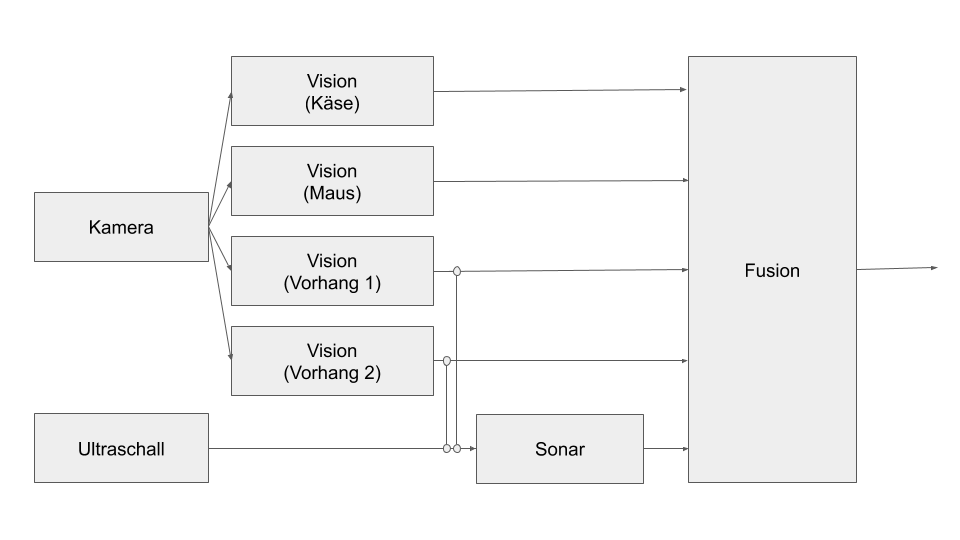
\includegraphics[scale=0.7]{media/struktur.png}
\end{figure}
%\bigskip\bigskip\bigskip\bigskip\bigskip\bigskip\bigskip\bigskip
%Diese Arbeit entstand mit Hilfe von B.Sc. Jan Baumgärtner, vielen dank dafür.
\newpage
% Festlegung Art der Zitierung - Havardmethode: Abkuerzung Autor + Jahr
\bibliography{lit}
\bibliographystyle{abbrv}
\end{document}
